\chapter{Tension Members}
Tension members are commonly used as bracing in trusses and elsewhere. They may be wires, rods, bars, structural shapes, etc.
\begin{figure}[H]
\centering
\footnotesize
\begin{tikzpicture}
\draw(0,-.4)rectangle(6,.4);
\draw[->](6.5,0)--++(1,0)node[right=3mm]{$N^*$};
\draw[->](-.5,0)--++(-1,0)node[left=3mm]{$N^*$};
\end{tikzpicture}
\end{figure}
\section{Strength Design Concept}\label{sec:tension}
The LRFD equation possesses the following form (\NZSSTEEL{\S~7.1}):
\begin{gather}
\begin{split}
%\sum\gamma_iE_i&\leqslant\phi{}R_n\\
%\text{Force}&\leqslant\text{Resistance}\\
N^*&\leqslant\phi{}N_t
\end{split}
\end{gather}
where
\begin{conditions}
N^*&factored summation of forces\\
N_t&nominal (ideal) tensile strength\\
\phi&strength reduction factor, for tension $\phi_t=\num{0.9}$
\end{conditions}

Failure is considered to occur as a result of either:
\begin{itemize}
\item \textbf{Excessive elongation}: yield over the \textbf{gross} area $A_g$\\
In this case, $N_t$ is determined by the gross area:
\begin{gather}\label{eq:tension_gross}
N_t=A_gf_y
\end{gather}
where
\begin{conditions}
A_g&gross cross section area\\
f_y&yield strength
\end{conditions}
\item \textbf{Sudden strength decrease}: facture over the \textbf{net} area $A_n$\\
In this case, $N_t$ is determined by the net area:
\begin{gather}\label{eq:tension_net}
N_t=0.85k_{te}A_nf_u
\end{gather}
where
\begin{conditions}
k_{te}&the correction factor for distribution of forces\\
A_n&net cross section area\\
f_u&tensile (ultimate) strength
\end{conditions}
\begin{figure}[H]
\centering
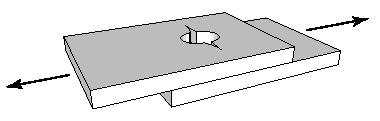
\includegraphics{PIC/CH03/NET}
\caption{Fracture over net area}
\end{figure}
\end{itemize}

Thus, to design a member in tension, one shall use the following criterion.
\begin{gather}
N^*\leqslant\min\left(\phi{}A_gf_y,~\phi{}0.85k_{te}A_nf_u\right).
\end{gather}
\begin{figure}[H]
\centering\footnotesize
\begin{tikzpicture}
\def\a{.4}\def\b{2}
\newcommand{\Bolt}{
\draw[fill=white](-\a,-\a)rectangle(\a,\a);
\draw(-.7*\a,-2.5*\a)rectangle(.7*\a,\a);
\draw(-1.4*\a,\a)rectangle(0,1.8*\a);
\draw(0,\a)rectangle(1.4*\a,1.8*\a);
\draw(-1.4*\a,-\a)rectangle(0,-1.8*\a);
\draw(0,-\a)rectangle(1.4*\a,-1.8*\a);
}
\draw(-\b,0)rectangle(1.5*\b,\a);
\draw(-1.5*\b,0)rectangle(\b,-\a);
\draw[->](1.6*\b,.5*\a)--++(1,0)node[right=3mm]{$N^*$};
\draw[->](-1.6*\b,-.5*\a)--++(-1,0)node[left=3mm]{$N^*$};
\setstructmech{convention=direction}
\Bolt
\begin{scope}[yshift=-3cm]
\draw(-1.5*\b,-1.5)rectangle(\b,1.5);
\draw[fill=white,fill opacity=.8](-\b,-1.2)rectangle(1.5*\b,1.2);
\draw[->](1.6*\b,0)--++(1,0)node[right=3mm]{$N^*$};
\draw[->](-1.6*\b,0)--++(-1,0)node[left=3mm]{$N^*$};
\draw[cc0066,ultra thick,dashed](0,1.2)--(0,-1.2)node[below=5mm]{$A_n$};
\draw[cc0066,ultra thick,dashed](1,1.2)--(1,-1.2)node[below=5mm]{$A_g$};
\node(0,0)[very thick,circle,draw,minimum size=8mm,fill=white]{};
\node[align=left]at(7,1){Note the top plate has smaller\\section width which governs.};
\begin{scope}[yshift=-3cm]
\begin{scope}[xshift=-2cm]
\draw[pattern=north west lines](-1.5,-.2)rectangle(1.5,.2)node[midway,below=7mm]{$A_n$};
\draw[fill=white](-.3,-.2)rectangle(.3,.2);
\end{scope}
\begin{scope}[xshift=2cm]
\draw[pattern=north west lines](-1.5,-.2)rectangle(1.5,.2)node[midway,below=7mm]{$A_g$};
\draw[|<->|](2,-.2)--++(0,.4)node[midway,right=2mm]{$t$};
\end{scope}
\end{scope}
\end{scope}
\end{tikzpicture}
\caption{Definitions of gross and net areas}
\end{figure}
\subsection{Definition of Net Area}
The \textbf{net} area of the section considers the \textbf{gross} areas of holes used in the member. For bolted members, the standard hole size $d_h$ is a function of the bolt diameter $d_f$ (\NZSSTEEL{\S~14.3.5.2.1}).
\begin{gather}\label{eq:dh}
d_h=\left\{
\begin{array}{ll}
d_f+\SI{2}{\mm},&d_f\leqslant\SI{24}{\mm},\\
d_f+\SI{3}{\mm},&d_f>\SI{24}{\mm}.
\end{array}
\right.
\end{gather}
\subsubsection{Unstaggered Holes}
According to \NZSSTEEL{\S~9.1.10.2}, for holes that are not staggered, the area to be deducted shall be the \textbf{maximum} summation of the areas of the holes in any cross sections that are perpendicular to the direction of the design action. For a cross section with $n$ holes of size $d_{h,i}$ of a plate of thickness $t$, the net area can be computed as
\begin{gather}\label{eq:unstaggered}
A_n=A_g-\sum_{i=1}^{n}d_{h,i}t_i.
\end{gather}
The calculated net area is indeed the \textbf{minimum} `net' area.
\subsubsection{Staggered Holes}
According to \NZSSTEEL{\S~9.1.10.3}, for staggered holes, the area to be deducted shall be the \textbf{greater} of:
\begin{enumerate}
\item the deduction of non-staggered holes,
\item the summation of the areas of all holes in any zig-zag line extending progressively across the member or part of the member.
\end{enumerate}
For a zig-zag line with $n$ holes and $m$ diagonal line segments, the net area shall be computed as follows.
\begin{gather}\label{eq:staggered}
A_n=A_g-\sum_{i=1}^{n}d_{h,i}t_i+\sum_{j=1}^{m}\frac{s_{p,j}^2t_j}{4s_{g,j}},
\end{gather}
in which
\begin{conditions}
s_{p}&staggered pitch, distance between hole centers measured \textbf{parallel} to the force direction\\
s_{g}&gauge length, distance between hole centers measured \textbf{perpendicular} to the force direction
\end{conditions}
\begin{figure}[H]
\centering
\footnotesize
\begin{tikzpicture}
\draw(2,0)rectangle(6,3);
\node[draw,circle,minimum size=3mm]at(5,2.5){};
\node[draw,circle,minimum size=3mm]at(4,1){};
\draw[dashed,cc0066,thick](5,3)--(5,2.5)--(4,1)--(4,0);
\draw[|<->|](3.5,1)--++(0,1.5)node[midway,fill=white]{$s_g$};
\draw[|<->|](4,.5)--++(1,0)node[midway,fill=white]{$s_p$};
\draw[->](6.5,1.5)--++(1,0)node[right=3mm]{$N^*$};
\draw[->](1.5,1.5)--++(-1,0)node[left=3mm]{$N^*$};
\end{tikzpicture}
\caption{Definition of gauge length and pitch}
\end{figure}

\eqsref{eq:unstaggered} is the simplified case of \eqsref{eq:staggered} with no diagonal line segments. For staggered layouts, the third term in \eqsref{eq:staggered} must be used. For any given bolt layouts, the governing net area shall be the \textbf{minimum} of all staggered and unstaggered cases. This is due to the fact that in a staggered layout, depending on pitch and gauge, an unstaggered section may have smaller net area than a staggered section.

If all holes have the same size $d_{h,i}=d_h$, and the plate thickness is uniform $t_i=t_j=t$, then it is possible to express the net area as $A_n=Lt$ with $L=b-nd_h+\sum_{j=1}^{m}\dfrac{s_{p,j}^2}{4s_{g,j}}$. The main task is to find the length of critical fracture line $L$.

\begin{exmp}
For the plate shown, assume the thickness is $t=\SI{12}{\mm}$ and the diameter of bolts is \SI{20}{\mm}, to compute the critial fracture line, both staggered and unstaggered cases need to be considered.
\begin{figure}[H]\centering
\footnotesize
\begin{tikzpicture}[x=1cm,y=1cm,ext/.pic={
\path[fill=exmpbg](-0.2,0)to[bend left](0,0.1)to[bend right](0.2,0.2)to(0.2,0)to[bend left](0,-0.1)to[bend right](-0.2,-0.2)--cycle;
\draw(-0.2,0)to[bend left](0,0.1)to[bend right](0.2,0.2) (0.2,0)to[bend left](0,-0.1)to[bend right](-0.2,-0.2);
}]
\newcommand{\StaggeredPlate}{
\draw[very thick](0,0)--++(0,3.55)--++(2.5,0)--pic{ext}++(0,-3.55)--cycle;
\draw(.7,.4)node[very thick,circle,inner sep=0,minimum size=4mm,draw]{}node[left=2mm]{$E$};
\draw(1.2,1.4)node[very thick,circle,inner sep=0,minimum size=4mm,draw]{}node[right=2mm]{$D$};
\draw(.7,2.15)node[very thick,circle,inner sep=0,minimum size=4mm,draw]{}node[left=2mm]{$C$};
\draw(1.2,3.15)node[very thick,circle,inner sep=0,minimum size=4mm,draw]{}node[right=2mm]{$B$};
\draw(1.2,0)node{\textbar}node[below right=1mm]{$G$};
\draw(.7,0)node{\textbar}node[below right=1mm]{$F$};
\draw(1.2,3.55)node{\textbar}node[above right=1mm]{$A$};
}
\begin{scope}[scale=1.2]
\StaggeredPlate
\draw[|<->|](.7,-.5)--++(.5,0)node[midway,fill=exmpbg,below=3mm]{$s_p=\num{50}$};
\draw[|<->|](-.5,0)--++(0,.4)node[midway,fill=exmpbg,left=2mm]{\num{40}};
\draw[|<->|](-.5,.4)--++(0,1)node[midway,fill=exmpbg]{$s_{g,DE}=\num{100}$};
\draw[|<->|](-.5,1.4)--++(0,.75)node[midway,fill=exmpbg]{$s_{g,CD}=\num{75}$};
\draw[|<->|](-.5,2.15)--++(0,1)node[midway,fill=exmpbg]{$s_{g,BC}=\num{100}$};
\draw[|<->|](-.5,3.14)--++(0,.4)node[midway,fill=exmpbg,left=2mm]{\num{40}};
\NodalForce{4.5,3.55/2}[N^*][N][N]
\end{scope}
\begin{scope}[xshift=5.5cm,yshift=2.73cm]
\StaggeredPlate
\draw(1.2,0)node{\textbar}node[below right=1mm]{$G$};
\draw(.7,0)node{\textbar}node[below right=1mm]{$F$};
\draw(1.2,3.55)node{\textbar}node[above right=1mm]{$A$};
\draw[cc0066,dashed,very thick](1.2,3.55)--++(0,-3.55);
\end{scope}
\begin{scope}[xshift=5.5cm,yshift=-2.02cm]
\StaggeredPlate
\draw(1.2,0)node{\textbar}node[below right=1mm]{$G$};
\draw(.7,0)node{\textbar}node[below right=1mm]{$F$};
\draw(1.2,3.55)node{\textbar}node[above right=1mm]{$A$};
\draw[cc0066,dashed,very thick](1.2,3.55)--++(0,-2.15)--++(-.5,-1)--++(0,-.4);
\end{scope}
\begin{scope}[xshift=10cm,yshift=2.73cm]
\StaggeredPlate
\draw(1.2,0)node{\textbar}node[below right=1mm]{$G$};
\draw(.7,0)node{\textbar}node[below right=1mm]{$F$};
\draw(1.2,3.55)node{\textbar}node[above right=1mm]{$A$};
\draw[cc0066,dashed,very thick](1.2,3.55)--(1.2,3.15)--(.7,2.15)--(1.2,1.4)--(1.2,0);
\end{scope}
\begin{scope}[xshift=10cm,yshift=-2.02cm]
\StaggeredPlate
\draw(1.2,0)node{\textbar}node[below right=1mm]{$G$};
\draw(.7,0)node{\textbar}node[below right=1mm]{$F$};
\draw(1.2,3.55)node{\textbar}node[above right=1mm]{$A$};
\draw[cc0066,dashed,very thick](1.2,3.55)--(1.2,3.15)--(.7,2.15)--(1.2,1.4)--(.7,.4)--(.7,0);
\end{scope}
\end{tikzpicture}
\end{figure}
\end{exmp}
\begin{solution}
The standard hole size $d_h=\SI{20}{\mm}+\SI{2}{\mm}=\SI{22}{\mm}$. The width $b=\SI{355}{\mm}$. The four cases considered are:
\begin{itemize}
\item Line ABDG --- Unstaggered
\begin{gather*}
L_{ABDG}=b-2d_h=\SI{355}{\mm}-2\times\SI{22}{\mm}=\SI{311}{\mm}.
\end{gather*}
\item Line ABDEF --- Staggered\\
There are three bolts and one diagonal line DE, for which $s_p=\SI{50}{\mm}$ and $s_g=\SI{100}{\mm}$.
\begin{gather*}
\begin{split}
L_{ABDEF}&=b-3d_h+\dfrac{s_p^2}{4s_g}\\&=\SI{355}{\mm}-3\times\SI{22}{\mm}+\dfrac{\left(\SI{50}{\mm}\right)^2}{4\times\SI{100}{\mm}}=\SI{295.3}{\mm}.
\end{split}
\end{gather*}
\item Line ABCDG --- Staggered\\
There are three bolts and two diagonal lines. For BC, $s_p=\SI{50}{\mm}$ and $s_g=\SI{100}{\mm}$. For CD, $s_p=\SI{50}{\mm}$ and $s_g=\SI{75}{\mm}$.
\begin{gather*}
\begin{split}
L_{ABCDG}&=b-3d_h+\sum\dfrac{s_p^2}{4s_g}\\&=\SI{355}{\mm}-3\times\SI{22}{\mm}+\dfrac{\left(\SI{50}{\mm}\right)^2}{4\times\SI{100}{\mm}}+\dfrac{\left(\SI{50}{\mm}\right)^2}{4\times\SI{75}{\mm}}=\SI{303.6}{\mm}.
\end{split}
\end{gather*}
\item Line ABCDEF --- Staggered\\
There are four bolts and three diagonal lines: BC, CD and DE.
\begin{gather*}
\begin{split}
L_{ABCDEF}&=b-4d_h+\sum\dfrac{s_p^2}{4s_g}\\&=\SI{355}{\mm}-4\times\SI{22}{\mm}+\dfrac{2\times\left(\SI{50}{\mm}\right)^2}{4\times\SI{100}{\mm}}+\dfrac{\left(\SI{50}{\mm}\right)^2}{4\times\SI{75}{\mm}}=\SI{287.8}{\mm}.
\end{split}
\end{gather*}
\end{itemize}
The governing case leads to the \textbf{minimum} net area $A_n=L_{ABCDEF}t=\SI{287.8}{\mm}\times\SI{12}{\mm}=\SI{3454}{\mm^2}$. In this example, since the plate is resisting $N^*$ applied on the right side, there is \textbf{no} need to consider cases such as ABCEF in which bolt at D has provided some resistance. The design of bolted connection will be introduced in Chapter \ref{ch:bolt}.
\end{solution}
\subsubsection{Angle Connection}
For angle connection, the gauge $s_g$ shall be taken as the sum of the back marks to each hole, less the leg thickness (\NZSSTEEL{Fig. 9.1.10.3(2)}).
\begin{figure}[H]
\centering
\footnotesize
\begin{tikzpicture}
\draw[pattern=north west lines](0,0)--(3,0)arc(0:90:.4)--(.4,.4)--(.4,2)arc(0:90:.4)--cycle;
\draw[fill=white](2,0)rectangle(2.4,.4);
\draw[fill=white](0,1.4)rectangle(.4,1.8);
\draw[dashed,ultra thick,cc0066](2.2,.2)-|(.2,1.6);
\draw[thick,cc0066,<-](.6,.3)--++(2,2)node[fill=white]{It's measured from \textbf{centre}!};
\draw[|<->|](0,-.5)--++(2.2,0)node[midway,fill=white]{$s_{g,1}$};
\draw[|<->|](-.5,0)--++(0,1.6)node[midway,fill=white]{$s_{g,2}$};
\draw[|<->|](0,2.6)--++(.4,0)node[midway,fill=white,above=2mm]{$t_2$};
\draw[|<->|](3.2,0)--++(0,.4)node[midway,fill=white,right=4mm]{$t_1$};
\draw[|<->|](0,-1)--++(.2,0)node[midway,fill=white,below=2mm]{$t_2/2$};
\draw[|<->|](-1,0)--++(0,.2)node[midway,fill=white,left=3mm]{$t_1/2$};
\draw[->](3.5,1)--++(2,0)node[midway,above]{fold out};
\begin{scope}[xshift=6cm,yshift=-.3cm]
\draw(0,0)rectangle(6,2);
\draw(0,2)rectangle(6,3);
\draw[dashed](0,1.8)--++(6,0)(0,2.2)--++(6,0);
\node[draw,circle,minimum size=3mm]at(5,2.5){};
\node[draw,circle,minimum size=3mm]at(4,1){};
\draw[dashed,cc0066,thick](5,3)--(5,2.5)--(4,1)--(4,0);
\draw[|<->|](3.5,1)--(3.5,2.5)node[midway,fill=white]{$s_g$};
\draw[|<->|](2.75,1)--(2.75,2.2)node[midway,fill=white]{$s_{g,1}$};
\draw[|<->|](2,2.5)--(2,1.8)node[midway,fill=white]{$s_{g,2}$};
\draw[|<->|](1.2,2)--(1.2,2.2)node[midway,fill=white,above=3mm]{$t_1/2$};
\draw[|<->|](.6,2)--(.6,1.8)node[midway,fill=white,below=3mm]{$t_2/2$};
\end{scope}
\end{tikzpicture}
\caption{Illustration of gauge of staggered layout in an angle}
\end{figure}
Essentially, the distance measured at the \textbf{centre} of thickness is evaluated. That is,
\begin{gather}
s_g=s_{g,1}+s_{g,2}-\dfrac{t_1+t_2}{2}.
\end{gather}
\subsection{Determination of Distribution Factor}
A correction factor $k_{te}$ is used to account for the concept of shear lag, or plane sections not remaining plane. This concept may be seen from the following examples.
\begin{figure}[H]
\centering
\footnotesize
\begin{tikzpicture}
\draw[thick](-.2,0)rectangle(.2,2);
\node at(0,2.5)[]{
\includegraphics[width=7mm]{PIC/CH03/BUG}};
\draw[dashed](-.5,-.5)--++(10,0);
\draw[thick,fill=black!20](-.2,-.5)rectangle(.2,-1.5);
\begin{scope}[xshift=1cm]
\draw[thick](-.5,0)rectangle(.5,2);
\node at(0,2.5)[]{
\includegraphics[width=7mm]{PIC/CH03/BUG}};
\draw[thick,fill=black!20](-.5,-.5)rectangle(.5,-1);
\end{scope}
\begin{scope}[xshift=6cm]
\draw[thick](-4,0)rectangle(4,2);
\node at(0,2.5)[]{
\includegraphics[width=7mm]{PIC/CH03/BUG}};
\draw[thick,fill=black!20](-4,-.5)--(-1,-.5)to[out=0,in=180](0,-.7)to[out=0,in=180](1,-.5)--(4,-.5);
\node at(4,-1){$\sigma$};
\end{scope}
\end{tikzpicture}
\end{figure}

In other connections, the same effect can be seen. Factors affecting shear lag are
\begin{itemize}
\item proportion of section connected;

It may be seen that the stress flow lines change direction and move together  concentrating stress.
\begin{figure}[H]
\centering
\footnotesize
\begin{tikzpicture}[scale=1,ext/.pic={
\path[fill=white](-0.2,0)to[bend left](0,0.1)to[bend right](0.2,0.2)to(0.2,0)to[bend left](0,-0.1)to[bend right](-0.2,-0.2)--cycle;
\draw(-0.2,0)to[bend left](0,0.1)to[bend right](0.2,0.2) (0.2,0)to[bend left](0,-0.1)to[bend right](-0.2,-0.2);
}]
\draw(2,-1.5)rectangle(-1,1.5);
\draw[fill=white](0,-1)rectangle(3,1);
\draw(-1,0)pic{ext};
\draw[line width=1.2mm](2,1)--(0,1)(2,-1)--(0,-1);
\UDL{4.5,-1}{4.5,1}{.5}
\foreach\x in{0,.2,.4,.6,.8,1}{
\draw(2*\x,1)to[out=-60+30*\x,in=180](3,.8*\x);
\draw(2*\x,-1)to[out=60-30*\x,in=180](3,-.8*\x);
}
\draw(2,1.7)|-++(-.2,.2)node[left]{A};
\draw(2,-1.7)|-++(-.2,-.2)node[left]{A};
\draw[fill=cc0066,opacity=.6](-2,-1)|-++(-1,2)node[above]{$f$}to[out=-90,in=90](-2.6,0)to[out=-90,in=90](-3,-1)--cycle;
\node at(-2.5,-1.5){section A};
\end{tikzpicture}
\end{figure}
\item length of weld or number of connects, more shear lag is expected with fewer connectors;
\begin{figure}[H]
\centering
\footnotesize
\begin{tikzpicture}[scale=1,ext/.pic={
\path[fill=white](-0.2,0)to[bend left](0,0.1)to[bend right](0.2,0.2)to(0.2,0)to[bend left](0,-0.1)to[bend right](-0.2,-0.2)--cycle;
\draw(-0.2,0)to[bend left](0,0.1)to[bend right](0.2,0.2) (0.2,0)to[bend left](0,-0.1)to[bend right](-0.2,-0.2);
}]
\draw(2,-1.5)rectangle(-1,1.5);
\draw[fill=white](1,-1)rectangle(3,1);
\draw(-1,0)pic{ext};
\draw[line width=1.2mm](2,1)--(1,1)(2,-1)--(1,-1);
\UDL{4.5,-1}{4.5,1}{.5}
\foreach\x in{0,.2,.4,.6,.8,1}{
\draw(1+\x,1)to[out=-60+30*\x,in=180](3,.8*\x);
\draw(1+\x,-1)to[out=60-30*\x,in=180](3,-.8*\x);
}
\draw(2,1.7)|-++(-.2,.2)node[left]{A};
\draw(2,-1.7)|-++(-.2,-.2)node[left]{A};
\draw[fill=cc0066,opacity=.6](-2,-1)|-++(-1,2)node[above]{$f$}to[out=-90,in=90](-2.2,0)to[out=-90,in=90](-3,-1)--cycle;
\node at(-2.5,-1.5){section A};
\end{tikzpicture}
\end{figure}
\item change in direction of stress due to section shape,  e.g., angle connected with fillet welds on both sides of one leg.
\begin{figure}[H]
\centering\footnotesize
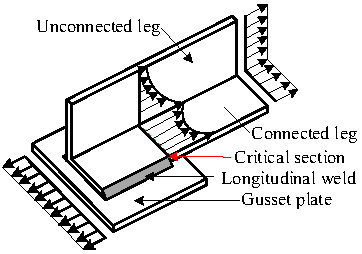
\includegraphics{PIC/CH03/SHEARLAG}
\caption{Shear lag in welded angle specimen \citep{Dhanuskar2021}}
\end{figure}
\begin{figure}[H]
\centering\footnotesize
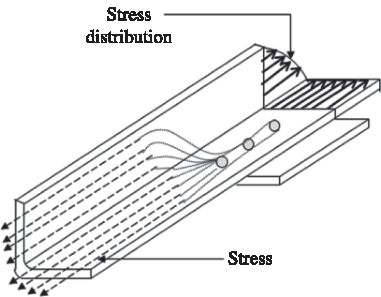
\includegraphics{PIC/CH03/BSL}
\caption{Shear lag in bolted angle specimen}
\end{figure}
\end{itemize}

The determination of $k_{te}$ is explained in \NZSSTEEL{\S~7.3}.

Some codes define an effective net area $A_e=k_{te}A_n$. We will use the AISC recommendations, because they are clearer, and more reasonable than the AS/NZS approach. They are given in \figref{fig:shear_lag} (\ANSI{Table D3.1}), where $U=k_{te}$.
\begin{figure}[p]
\centering
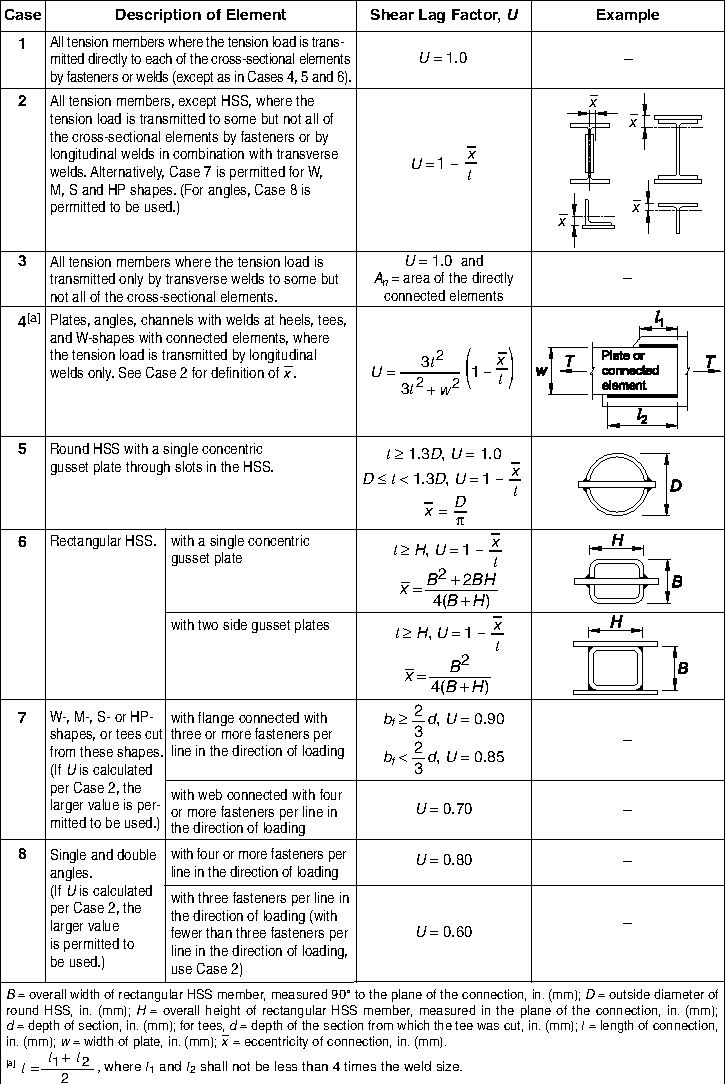
\includegraphics[width=.99\textwidth]{PIC/CH03/SHEAR.LAG}
\caption{Shear lag factors for connections to tension members}
\label{fig:shear_lag}
\end{figure}
\section{Tension Member Slenderness Limitations}
Most codes do not have any requirements for slenderness. However, undesired flutter (or vibration) of slender tension members have been observed in some situations. The AISC-LRFD code makes the following recommendations (\ANSI{\S~D1}): For members designed on the basis of tension, the slenderness ratio, $L/r$, preferably \textbf{should not exceed 300}. This suggestion does not apply to rods or hangers in tension.
\begin{exmp}\href{run:./WORKSHEET/CH03/EX3.ATUC.sm}{Worksheet}
Axial Tension Example --- Slender UC

Choose a \SI{8}{\meter} long UC section to carry $G=\SI{880}{\kn}$ and $Q=\SI{1200}{\kn}$ respectively with Grade 300 steel.
\end{exmp}
\begin{solution}
Assume $f_y=\SI{280}{\mpa}$, the factored tension force is given by the critical load combination,
\begin{align*}
N^*_t=\sum\gamma_iE_i&=1.2G+1.5Q\\
&=1.2\times\SI{880}{\kn}+1.5\times\SI{1200}{\kn}\\
&=\SI{2856}{\kn}.
\end{align*}
LRFD requires the following for material yielding on the gross area.
\begin{align*}
N^*_t&\leqslant\phi{}N_t\\
&\leqslant\phi{}A_gf_y,\\
A_g&\geqslant\dfrac{N^*_t}{\phi{}f_y}=\SI{11330}{\mm^2}.
\end{align*}
Try 250UC89.5,
\begin{gather*}
A_g=\SI{11400}{\mm^2}>\SI{11330}{\mm^2}.
\end{gather*}
Check slenderness requirement, considering the minimum $r$ value:
\begin{gather*}
\dfrac{L}{r_{min}}=\dfrac{L}{r_y}=\dfrac{8000}{65.5}=\num{122.7}<\num{300},\qquad\text{Okay.}
\end{gather*}
Since $t_f=\SI{17.3}{\mm}>\SI{17}{\mm}$, the assumed yield stress $f_y=\SI{280}{\mpa}$ is correct, see, \tabref{tab:ys}. Thus, a 250UC89.5 section works. Alternatively, the next section, 310UC96.8, also works but its heavier.

Note:
\begin{itemize}
\item The critical loading actions need to be combined for ultimate limit states (left hand side of the equation).
\item Remember slenderness may impose additional requirements.
\end{itemize}
\end{solution}

\begin{exmp}\href{run:./WORKSHEET/CH03/EX3.ATBC.sm}{Worksheet}
Axial Tension Example --- Staggered Bolt Connection

Assuming Grade 300 steel and $\phi~\SI{12}{\mm}$ bolts, the thickness of top plate is \SI{12}{\mm}, what is the maximum factored force (or design strength) in tension of the top plate shown below?
\begin{figure}[H]
\footnotesize
\begin{tikzpicture}[scale=1.4,x=1cm,y=1cm,ext/.pic={
\path[fill=exmpbg](-0.2,0)to[bend left](0,0.1)to[bend right](0.2,0.2)to(0.2,0)to[bend left](0,-0.1)to[bend right](-0.2,-0.2)--cycle;
\draw(-0.2,0)to[bend left](0,0.1)to[bend right](0.2,0.2) (0.2,0)to[bend left](0,-0.1)to[bend right](-0.2,-0.2);
}]
\draw[very thick](0,0)--++(0,2.3)--++(2.5,0)--pic{ext}++(0,-2.3)--cycle;
\draw(.7,.5)node[very thick,circle,inner sep=0,minimum size=4mm,draw]{}node[left=2mm]{$E$};
\draw(.7,1.15)node[very thick,circle,inner sep=0,minimum size=4mm,draw]{}node[left=2mm]{$D$};
\draw(.7,1.8)node[very thick,circle,inner sep=0,minimum size=4mm,draw]{}node[left=2mm]{$C$};
\draw(1.4,.5)node[very thick,circle,inner sep=0,minimum size=4mm,draw]{}node[right=2mm]{$F$};
\draw(1.4,1.8)node[very thick,circle,inner sep=0,minimum size=4mm,draw]{}node[right=2mm]{$B$};
\draw(1.4,0)node{\textbar}node[below right=1mm]{$G$};
\draw(1.4,2.3)node{\textbar}node[above right=1mm]{$A$};
\draw[|<->|](.7,-.25)--++(.7,0)node[midway,fill=exmpbg]{\num{70}};
\draw[|<->|](-.5,0)--++(0,.5)node[midway,fill=exmpbg]{\num{50}};
\draw[|<->|](-.5,.5)--++(0,.65)node[midway,fill=exmpbg]{\num{65}};
\draw[|<->|](-.5,1.15)--++(0,.65)node[midway,fill=exmpbg]{\num{65}};
\draw[|<->|](-.5,1.8)--++(0,.5)node[midway,fill=exmpbg]{\num{50}};
\draw[very thick](2,0)|-(-1,-.4)|-(2,2.7)--++(0,-.4);
\draw[dashed](2,0)--++(0,2.3);
\NodalForce{5,1.15}[N^*][N][N]
\end{tikzpicture}
\end{figure}
\end{exmp}
\begin{solution}
A member subjected to an axial tension force shall satisfy:
\begin{gather*}
N^*\leqslant\min\left(\phi{}A_gf_y,~\phi{}0.85k_{te}A_nf_u\right).
\end{gather*}
In this case, $k_{te}=1$. The overall width $b$ is
\begin{gather*}
b=2\times\SI{50}{\mm}+2\times\SI{65}{\mm}=\SI{230}{\mm}.
\end{gather*}
The standard hole size is
\begin{gather*}
d_h=\SI{12}{\mm}+\SI{2}{\mm}=\SI{14}{\mm}.
\end{gather*}
Because $t=\SI{12}{\mm}>\SI{11}{\mm}$, for Grade 300 steel, $f_y=\SI{310}{\mpa}$ and $f_u=\SI{430}{\mpa}$.

For gross area,
\begin{gather*}
A_gf_y=btf_y=\SI{230}{\mm}\times\SI{12}{\mm}\times\SI{310}{\mpa}=\SI{855.6}{\kn}.
\end{gather*}
For net area, find critical fracture line first. When fracture line is $ABFG$,
\begin{gather*} L_{ABFG}=b-2d=\SI{230}{\mm}-2\times\SI{14}{\mm}=\SI{202}{\mm}.\qquad\rightarrow\qquad\text{critical}
\end{gather*}
When fracture line is $ABDFG$,
\begin{gather*}
L_{ABDFG}=\SI{230}{\mm}+2\times\dfrac{\left(\SI{70}{\mm}\right)^2}{4\times\SI{65}{\mm}}-3\times\SI{14}{\mm}=\SI{225.7}{\mm}.
\end{gather*}
\begin{figure}[H]\centering\footnotesize
\begin{tikzpicture}[scale=1,x=1cm,y=1cm,ext/.pic={
\path[fill=exmpbg](-0.2,0)to[bend left](0,0.1)to[bend right](0.2,0.2)to(0.2,0)to[bend left](0,-0.1)to[bend right](-0.2,-0.2)--cycle;
\draw(-0.2,0)to[bend left](0,0.1)to[bend right](0.2,0.2) (0.2,0)to[bend left](0,-0.1)to[bend right](-0.2,-0.2);
}]
\draw(0,0)--++(0,2.3)--++(2.5,0)--pic{ext}++(0,-2.3)--cycle;
\draw(.7,.5)node[very thick,circle,inner sep=0,minimum size=4mm,draw]{};
\draw(.7,1.15)node[very thick,circle,inner sep=0,minimum size=4mm,draw]{};
\draw(.7,1.8)node[very thick,circle,inner sep=0,minimum size=4mm,draw]{};
\draw(1.4,.5)node[very thick,circle,inner sep=0,minimum size=4mm,draw]{};
\draw(1.4,1.8)node[very thick,circle,inner sep=0,minimum size=4mm,draw]{};
\draw(1.4,0)node{\textbar};
\draw(1.4,2.3)node{\textbar};
\draw[cc0066,dashed,very thick](1.4,0)--(1.4,2.3);
\begin{scope}[xshift=6cm]
\draw(0,0)--++(0,2.3)--++(2.5,0)--pic{ext}++(0,-2.3)--cycle;
\draw(.7,.5)node[very thick,circle,inner sep=0,minimum size=4mm,draw]{};
\draw(.7,1.15)node[very thick,circle,inner sep=0,minimum size=4mm,draw]{};
\draw(.7,1.8)node[very thick,circle,inner sep=0,minimum size=4mm,draw]{};
\draw(1.4,.5)node[very thick,circle,inner sep=0,minimum size=4mm,draw]{};
\draw(1.4,1.8)node[very thick,circle,inner sep=0,minimum size=4mm,draw]{};
\draw(1.4,0)node{\textbar};
\draw(1.4,2.3)node{\textbar};
\draw[cc0066,dashed,very thick](1.4,0)--(1.4,.5)--(.7,1.15)--(1.4,1.8)--(1.4,2.3);
\end{scope}
\end{tikzpicture}
\end{figure}
Thus,
\begin{gather*}
A_n=L_{ABFG}t=\SI{202}{\mm}\times\SI{12}{\mm}=\SI{2424}{\mm^2}.
\end{gather*}
Then,
\begin{gather*}
0.85k_{te}A_nf_u=0.85\times1\times\SI{2424}{\mm^2}\times\SI{430}{\mpa}=\SI{886}{\kn}.
\end{gather*}
The maximum factored force is then
\begin{gather*}
N^*\leqslant\min\left(0.9\times\SI{855.6}{\kn},~0.9\times\SI{886}{\kn}\right)=\SI{770}{\kn}.
\end{gather*}
\begin{flushright}
$N^*=\SI{770}{\kn}$
\end{flushright}
\end{solution}
For connected members, both failure mechanisms need to be calculated. This applies to not only bolted connection with area reduction, but also other types of connections.

\begin{exmp}\href{run:./WORKSHEET/CH03/EX3.ATAC.sm}{Worksheet}
Axial Tension Example --- Angle Connection

Use Grade 300 steel, design a \SI{2.7}{\meter} single angle tension member connected to a plate with one leg (long leg if UA) using 5 M20 ($\phi\SI{20}{\mm}$) class 8.8 bolts in a line, with one at each section. Let $G=\SI{130}{\kn}$ and $Q=\SI{190}{\kn}$.

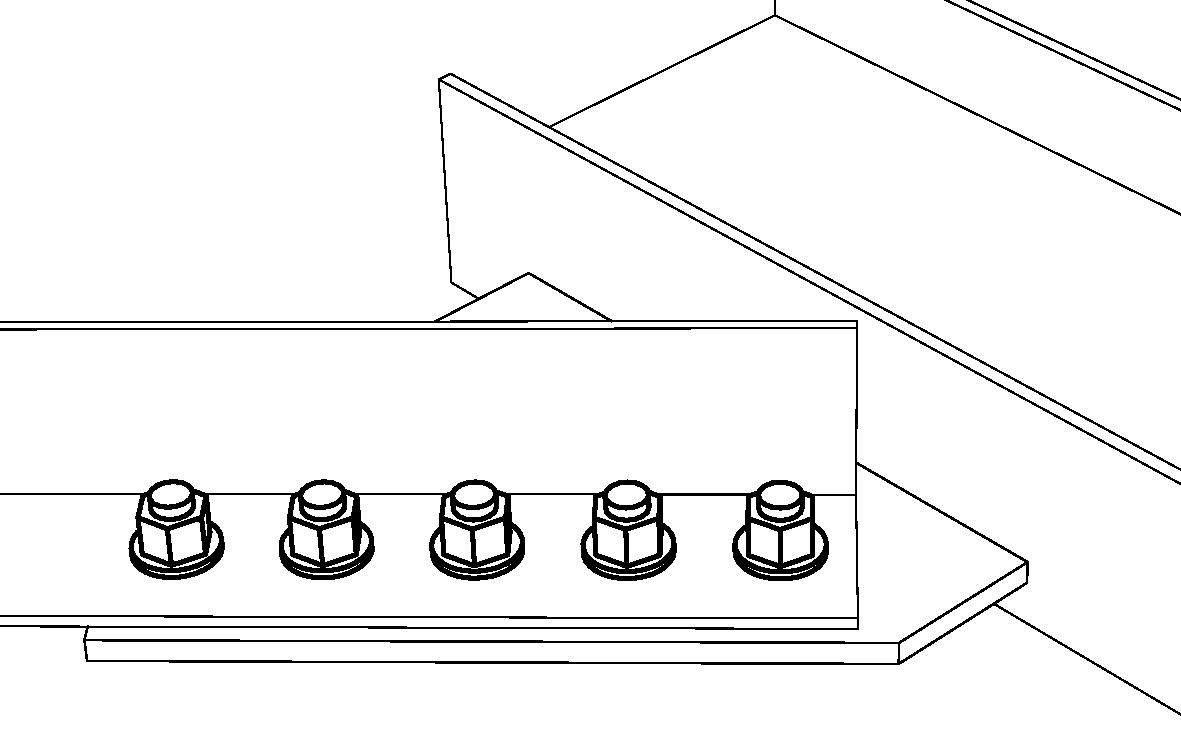
\includegraphics[width=7cm]{PIC/CH03/ANGLE}
\end{exmp}
\begin{solution}
The critical combination is
\begin{gather*}
N^*_t=\max\left(1.35G,~1.2G+1.5Q\right)=\SI{441}{\kn}.
\end{gather*}
Assume $f_y=\SI{320}{\mpa}$, the minimum gross area is
\begin{gather*}
A_g\geqslant\dfrac{N^*_t}{\phi{}f_y}=\dfrac{\SI{441}{\kn}}{0.9\times\SI{320}{\mpa}}=\SI{1531}{\mm^2}.
\end{gather*}
According to case 8 in \figref{fig:shear_lag}, $k_{te}=0.8$, the minimum net area is
\begin{gather*}
A_n\geqslant\dfrac{N^*_t}{\phi{}0.85k_{te}f_u}=\dfrac{\SI{441}{\kn}}{0.9\times0.85\times0.8\times\SI{440}{\mpa}}=\SI{1638}{\mm^2}.
\end{gather*}
Thus the net area governs. Try the following sections.
\begin{table}[H]
\centering\small
\begin{tabular}{lccccc}
	\toprule
	Section                        & $A_g$ & $t$ & $r_{min}$ & $A_n$  &      \\ \midrule
	125\texttimes75\texttimes10UA  & 1810  & 9.5 &   16.2    &  1601  & N.G. \\
	100\texttimes100\texttimes10EA & 1810  & 9.5 &   19.6    &  1601  & N.G. \\
	125\texttimes90\texttimes8UA   & 1820  & 7.8 &   19.7    & 1648.4 & Okay \\
	125\texttimes125\texttimes8EA  & 1900  & 7.8 &   24.8    & 1728.4 & Okay \\
	125\texttimes90\texttimes10UA  & 2200  & 9.5 &   19.6    &  1991  & Okay \\
	100\texttimes100\texttimes12EA & 2260  & 12  &   19.5    &  1996  & Okay \\ \bottomrule
\end{tabular}
\end{table}
Thus use 125\texttimes90\texttimes8UA. The thickness is smaller than \SI{11}{\mm}, thus the assumed yield stress is appropriate for Grade 300 steel.
\begin{flushright}
Use 125\texttimes90\texttimes8UA
\end{flushright}
\end{solution}

\begin{exmp}\href{run:./WORKSHEET/CH03/EX3.BFUC.sm}{Worksheet}
Axial Tension Example --- Bolted Flange UC

Find the size of UC member carrying axial loads $G=\SI{270}{\kn}$, $Q=\SI{400}{\kn}$ and $W=\SI{45}{\kn}$ using Grade 300 steel. The spacing of bolts is \SI{80}{\mm} along the direction of axial force. Note bolted connections apply to both sides of the member.
\begin{figure}[H]
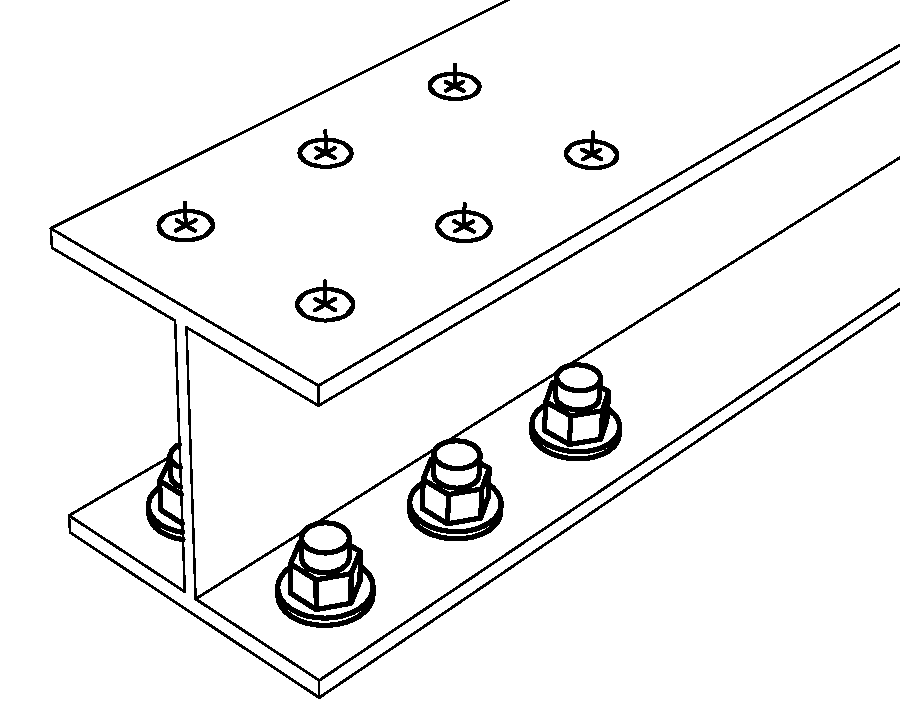
\includegraphics[width=7cm]{PIC/CH04/UC}

\begin{tikzpicture}[ext/.pic={
\path[fill=exmpbg](-0.2,0)to[bend left](0,0.1)to[bend right](0.2,0.2)to(0.2,0)to[bend left](0,-0.1)to[bend right](-0.2,-0.2)--cycle;
\draw(-0.2,0)to[bend left](0,0.1)to[bend right](0.2,0.2) (0.2,0)to[bend left](0,-0.1)to[bend right](-0.2,-0.2);
}]
\draw[dashed](7,-.07)rectangle(-7,.07);
\draw[very thick](7,-1)--pic{ext}++(0,2)--++(-14,0)--pic{ext}++(0,-2)--cycle;
\begin{scope}[rotate around={45:(0,0)}]
\draw[->,ultra thick](7.5,0)--++(2,0)node[above]{$G$, $Q$, $W$};
\draw[dashed](3,-.07)rectangle(7,.07);
\draw[very thick](3,-1)--++(4,0)--pic{ext}++(0,2)--++(-4,0)--cycle;
\end{scope}
\begin{scope}[rotate around={135:(0,0)}]
\draw[dashed](3,-.07)rectangle(7,.07);
\draw[very thick](3,-1)--++(4,0)--pic{ext}++(0,2)--++(-4,0)--cycle;
\end{scope}
\draw[very thick,fill=exmpbg,fill opacity=.8](5,-1)--++(0,4)--++(-2,2)--++(-6,0)--++(-2,-2)--++(0,-4)--cycle;
\foreach\x in{-4,-2,0,2,4}{
\foreach\y in{-.5,.5}\node at(\x,\y)[circle,draw]{};
}
\begin{scope}[rotate around={45:(0,0)}]
\node at(3.5,-.5)[circle,draw]{};
\node at(3.5,.5)[circle,draw]{};
\node at(4.3,-.5)[circle,draw]{};
\node at(4.3,.5)[circle,draw]{};
\node at(5.1,-.5)[circle,draw]{};
\node at(5.1,.5)[circle,draw]{};
\draw[ultra thick,cc0066](4.3,0)circle(2.2cm);
\end{scope}
\begin{scope}[rotate around={135:(0,0)}]
\node at(3.5,-.5)[circle,draw]{};
\node at(3.5,.5)[circle,draw]{};
\node at(4.3,-.5)[circle,draw]{};
\node at(4.3,.5)[circle,draw]{};
\node at(5.1,-.5)[circle,draw]{};
\node at(5.1,.5)[circle,draw]{};
\end{scope}
\end{tikzpicture}
\end{figure}
\end{exmp}
\begin{solution}
The demand can be obtained via combinations.
\begin{align*}
N^*_t&=\max\left(1.35G,~1.2G+1.5Q,~1.2G+\psi_cQ+W\right)\\
&=\max\left(\SI{364.5}{\kn},~\SI{924}{\kn},~\SI{529}{\kn}\right)\\
&=\SI{924}{\kn}.
\end{align*}
Assume $f_y=\SI{320}{\mpa}$, for yielding on gross area,
\begin{gather*}
A_g\geqslant\dfrac{N^*_t}{\phi{}f_y}=\dfrac{\SI{924}{\kn}}{0.9\times\SI{320}{\mpa}}=\SI{3208}{\mm^2}.
\end{gather*}
Try 150UC30.0, $A_g=\SI{3860}{\mm^2}$ and $t_f=\SI{9.4}{\mm}$. Since for each net section, there are 2 bolts per flange, totalling 4, the net area is
\begin{gather*}
A_n=A_g-4t_fd_h=\SI{3860}{\mm^2}-4\times\SI{9.4}{\mm}\times\SI{22}{\mm}=\SI{3033}{\mm^2}.
\end{gather*}
Since there are three bolts in a line and $b_f>\dfrac{2}{3}d$, from \figref{fig:shear_lag}, $k_{te}=0.9$ according to case 7. Thus for fracture on net area,
\begin{gather*}
\phi0.85k_{te}A_nf_y=0.9\times0.85\times0.9\times\SI{3033}{\mm^2}\times\SI{440}{\mpa}=\SI{919}{\kn}.
\end{gather*}
The difference is only \SI{0.5}{\percent}. Considering the ultimate strength would be greater, 150UC30.0 is okay.

Use case 2 in \tabref{fig:shear_lag} to recheck the example, from which,
\begin{gather*}
k_{te}=1-\dfrac{\bar{x}}{l}.
\end{gather*}
Since bolts are in both flanges, axial forces from half section goes to bolts on each side. Consider half section only, find eccentricity $\bar{x}$,

\begin{minipage}{6cm}
\centering\begin{tikzpicture}[x=1cm,y=1cm,scale=.5]
\draw[pattern=north west lines](-.25,0)rectangle(.25,4);
\draw[pattern=north west lines](-2.5,4)rectangle(2.5,4.5);
\draw[|<->|](3,-4)--++(0,8)node[midway,fill=exmpbg]{$d_1=138.8$};
\draw[|<->|](3,4)--++(0,.5)node[midway,fill=exmpbg,right=3mm]{$t_f=9.4$};
\draw[|<->|](-.25,-5)--++(.5,0)node[midway,fill=exmpbg,below=3mm]{$t_w=6.6$};
\draw[|<->|](-2.5,5.5)--++(5,0)node[midway,fill=exmpbg]{$b_f=153$};
\draw[dashed](-.25,-4)rectangle(.25,4);
\draw[dashed](-2.5,-4.5)rectangle(2.5,-4);
\draw[|->](-3,4.5)--++(0,-2)node[below]{$x$};
\draw[draw,fill=exmpbg](-1.75,4)rectangle(-1.25,4.5);
\draw[draw,fill=exmpbg](1.75,4)rectangle(1.25,4.5);
\end{tikzpicture}
\end{minipage}
\begin{minipage}{.99\linewidth-6cm}
\begin{align*}
\bar{x}&=\dfrac{\sum{}x_iA_i}{\sum{}A_i}\\&=\dfrac{\left(b_f-t_w\right)\cdot{}t_f\cdot{}t_f/2+t_w\cdot{}d/2\cdot{}d/4}{A_g/2}\\
&=\dfrac{\left(153-6.6\right)\cdot{}9.4\cdot{}4.7+6.6\cdot{}78.8\cdot{}39.4}{1930}\si{\mm}\\
&=\SI{13.97}{\mm}.
\end{align*}
The total length of connection is $l=2\times\SI{80}{\mm}=\SI{160}{\mm}$,
\begin{align*}
k_{te}&=1-\dfrac{\bar{x}}{l}\\
&=1-\dfrac{\SI{13.97}{\mm}}{\SI{160}{\mm}}\\
&=0.913.
\end{align*}
\end{minipage}

Thus,
\begin{gather*}
\phi0.85k_{te}A_nf_u=0.9\times0.85\times0.913\times\SI{3033}{\mm^2}\times\SI{440}{\mpa}=\SI{932}{\kn}>\SI{924}{\kn}.
\end{gather*}

The general method (case 2) is less conservative than the specific one (case 7) in this case.
\begin{flushright}
Use 150UC30.0
\end{flushright}
\begin{figure}[H]
\centering
\footnotesize
\begin{tikzpicture}[ext/.pic={
\path[fill=exmpbg](-0.2,0)to[bend left](0,0.1)to[bend right](0.2,0.2)to(0.2,0)to[bend left](0,-0.1)to[bend right](-0.2,-0.2)--cycle;
\draw(-0.2,0)to[bend left](0,0.1)to[bend right](0.2,0.2) (0.2,0)to[bend left](0,-0.1)to[bend right](-0.2,-0.2);
}]
\draw[dashed](0,-.07)rectangle(7,.07);
\draw[very thick](0,-1)--++(7,0)--pic{ext}++(0,2)--++(-7,0)--cycle;
\node at(1,-.5)[circle,draw]{};
\node at(1,.5)[circle,draw]{};
\node at(3,-.5)[circle,draw]{};
\node at(3,.5)[circle,draw]{};
\node at(5,-.5)[circle,draw]{};
\node at(5,.5)[circle,draw]{};
\draw[|<->|](0,1.3)--++(1,0)node[midway,fill=exmpbg]{40};
\draw[|<->|](1,1.3)--++(2,0)node[midway,fill=exmpbg]{80};
\draw[|<->|](3,1.3)--++(2,0)node[midway,fill=exmpbg]{80};
\draw[cc0066,very thick,dashed](5,-1.5)--++(0,3.5)node[fill=exmpbg]{potential failure plane};
\end{tikzpicture}
\end{figure}
\end{solution}

\begin{exmp}
Sag rods, threaded over their whole length, are to be designed to support purlins parallel to the roof surface as shown below. This is because purlins are strong in bending about their major axis, but they are weak about their minor axis. To prevent possible rod damage during construction, use a minimum diameter of \SI{16}{\mm} and to prevent flutter, use $L/d<500$. Assume Grade 300 steel.
\begin{figure}[H]
\centering
\tiny
\begin{tikzpicture}[scale=.6,spy using outlines={circle,magnification=4,size=3cm,connect spies}]
\draw(15,6)circle(8mm);
\draw[fill=black](15,6)circle(6mm);
\draw[fill=black](15-.8,6)to[out=80,in=180](15,6.6)--++(0,-.3)to[out=120,in=50]cycle;
\node[align=center]at(15,7.5){The rod is threaded such that\\$A_n$ is smaller than $A_g$.};
\draw(0,0)--++(21.6,0)--++(-10.8,3.6)--cycle;
\dimline[extension start length=0,extension end length=0]{($(21.6,0)+(.5,1.5)$)}{($(10.8,3.6)+(.5,1.5)$)}{\SI{11.38}{\meter}}
\dimline[extension start length=0,extension end length=0]{(-1,0)}{(-1,3.6)}{\SI{3.6}{\meter}}
\draw(3.6,0)--++(0,1.2)--(7.2,0)--++(0,2.4)--(10.8,0)--++(3.6,2.4)--++(0,-2.4)--++(3.6,1.2)--++(0,-1.2);
\draw(10.8,0)--++(0,3.6);
\dimline[extension start length=0,extension end length=0]{(0,-1)}{(21.6,-1)}{$6\times\SI{3.6}{\meter}=\SI{21.6}{\meter}$}
\draw[red](10.8-.3,4)--++(.6,0);
\spy[blue]on(10.8*.6,4*.6)in node at(5,8);
\begin{scope}[rotate=18.435,yshift=10]
\draw(0,.4)--++(1.0541*10.8+.25,0);
\foreach \x in {0,1.8,3.6,...,11}{
\draw(1.0541*\x-.3,-.2)--++(.3,0)--++(0,.4)--++(-.3,0);
}
\foreach \x in {0,3.6,7.2}{\draw(\x*1.0541-.1,.1)--++(1.8*1.0541+.2,0);}
\foreach \x in {1.8,5.4,9}{\draw(\x*1.0541-.1,-.1)--++(1.8*1.0541+.2,0);}
\draw[<-](3.6,.25)--++(-1,2)node[fill=exmpbg]{purlins (150PFC)};
\draw[<-](7.2,.5)--++(-1,2)node[fill=exmpbg]{clay cladding};
\end{scope}
\begin{scope}[yscale=1,xscale=-1,xshift=-21.6cm]
\begin{scope}[rotate=18.435,yshift=10]
\draw(0,.4)--++(1.0541*10.8+.25,0);
\foreach \x in {0,1.8,3.6,...,11}{
\draw(1.0541*\x-.3,-.2)--++(.3,0)--++(0,.4)--++(-.3,0);
}
\foreach \x in {0,3.6,7.2}{\draw(\x*1.0541-.1,.1)--++(1.8*1.0541+.2,0);}
\foreach \x in {1.8,5.4,9}{\draw(\x*1.0541-.1,-.1)--++(1.8*1.0541+.2,0);}
\end{scope}
\end{scope}
\node at(10.8,-2){Elevation};
\begin{scope}[yshift=-10cm]
\draw(0,0)rectangle(21.6,6.6);
\foreach \x in {2.2,4.4}\draw[dashed,very thin](0,\x)--++(21.6,0);
\foreach \x in {1.8,3.6,...,21.6}\draw(\x,0)--++(0,6.6);
\foreach \x in {0,3.6,7.2,...,21}{
\foreach \y in {2.2,4.4}{
\draw(\x-.1,\y-.1)--++(1.8+.2,0);
\draw(\x-.1+1.8,\y+.1)--++(1.8+.2,0);
}}
\dimline[extension start length=0,extension end length=0]{(-1,0)}{(-1,6.6)}{\SI{6.6}{\meter}}
\draw[very thick](10.8,0)--++(0,6.6);
\draw[<-](11,.4)--++(1,-1)node[fill=exmpbg]{gable purlins};
\draw[<-](8,4.6)--++(-1,1)node[fill=exmpbg]{sag rods};
\draw[<-](2,.4)--++(1,-1)node[fill=exmpbg]{purlins};
\draw[<-](5.6,.4)--++(1,-1)node[fill=exmpbg]{purlins};
\draw[pattern=north west lines](10.8,3.3)rectangle++(10.8,2.2);
\dimline[extension start length=0,extension end length=0]{(22.6,3.3)}{(22.6,5.5)}{tributary\\width}
\draw[<-](13,5)--++(1,1)node[fill=exmpbg]{tributary area};
\draw[<-](22,6.6)--++(1,0)node[fill=exmpbg]{truss};
\draw[<-](22,0)--++(1,0)node[fill=exmpbg]{truss};
\node at(10.8,-2){Plan};
\end{scope}
\end{tikzpicture}
\end{figure}
\end{exmp}
\begin{solution}
The rods are to be threaded such that $A_n=0.75A_g=0.75\times\dfrac{\pi{}d^2}{4}$. Since they are threaded over their whole length we only need to consider fracture,
\begin{gather*}
\phi{}N_t=0.9\times0.95\times{}k_{te}A_nf_u\geqslant{}N^*_t.
\end{gather*}
This gives
\begin{gather*}
\begin{split}
d(\si{\meter})&\geqslant\sqrt{\dfrac{4\times{}N^*_t}{0.9\times0.85\times{}k_{te}\times{}f_u\times0.75\times\pi{}}}\\&=\sqrt{\dfrac{4\times{}N^*_t}{0.9\times0.85\times{}1\times{}\SI{440}{\mpa}\times0.75\times\pi{}}}=\num{7.102e-5}\sqrt{N^*_t(\si{\newton})}.
\end{split}
\end{gather*}

We proceed to find $N^*$ on the member.
\begin{enumerate}
\item Clay roofing: \SI{800}{\pascal} on flat roof, i.e., on flat roof, weight is \SI{800}{\pascal}. On sloping roof, the weight per horizontal distance is
\begin{gather*}
\dfrac{\SI{800}{\pascal}}{\cos\alpha}=\dfrac{\sqrt{10}}{3}\times\SI{800}{\pascal}=\SI{843.3}{\pascal}.
\end{gather*}
\begin{figure}[H]
\centering\footnotesize
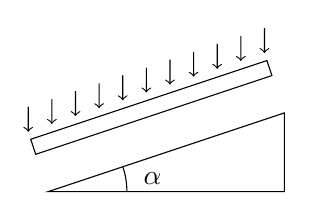
\begin{tikzpicture}
\draw(0,0)--++(3,0)--++(0,1)--cycle;
\draw(1,0)arc(0:18.435:1)node[midway,right=1mm]{$\alpha$};
\dimline[extension start length=0,extension end length=0]{(0,-.5)}{(3,-.5)}{3}
\dimline[extension start length=0,extension end length=0]{(3.5,0)}{(3.5,1)}{1}
\begin{scope}[rotate=18.435]
\draw(0,.5)rectangle++(3*1.0541,.2);
\foreach \x in {0,.3,.6,...,3.1}{
\draw[<-](\x*1.0541,.8)--++(.1,.3);}
\end{scope}
\end{tikzpicture}
\end{figure}
\item Snow pressure: \SI{1600}{\pascal} (vertical)
\item Purlin equivalent force: 150PFC has a linear density of \SI{17.7}{\kilogram\per\meter}, the horizontal spacing is \SI{1.8}{\meter}, this gives
\begin{gather*}
\dfrac{\SI{17.7}{\kilogram\per\meter}\times\SI{9.81}{\newton\per\kilogram}}{\SI{1.8}{\meter}}=\SI{96.5}{\pascal}.
\end{gather*}
\end{enumerate}
Collecting those terms, the design action
\begin{gather*}
\begin{split}
N^*_{v,Pa}&=1.2G+S\\&=1.2\times\left(\SI{843.3}{\pascal}+\SI{96.5}{\pascal}\right)+\SI{1600}{\pascal}=\SI{2728}{\pascal}
\end{split}
\end{gather*}

The equivalent total vertical force acting on sag rod is computed by accounting for tributary area. This leads to
\begin{gather*}
N^*_{v,kN}=\SI{2728}{\pascal}\times\SI{10.8}{\meter}\times\SI{6.6}{\meter}/3=\SI{64.8}{\kilo\newton}.
\end{gather*}

The critical tension force in sag rod is
\begin{gather*}
N^*_t=N^*_{v,kN}\sin\alpha=\SI{64.8}{\kilo\newton}\times\dfrac{1}{\sqrt{10}}=\SI{20.5}{\kn}.
\end{gather*}
\begin{figure}[H]
\centering\footnotesize
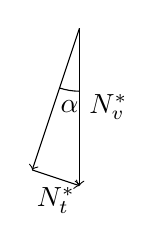
\begin{tikzpicture}[scale=.2,rotate=90]
\draw(6,0)arc(180:180-18.435:4)node[midway,below]{$\alpha$};
\draw[<-](0,0)--++(10,0)node[midway,right]{$N^*_v$};
\draw[->](10,0)--++(-9,3);
\draw[<-](0,0)--++(1,3)node[midway,below]{$N^*_t$};
\end{tikzpicture}
\end{figure}

Thus the minimum diameter is
\begin{gather*}
d=\num{7.102e-5}\sqrt{20500}=\SI{}{\meter}=\SI{1.017e-2}{\meter}=\SI{10.17}{\mm}\le\SI{16}{\mm}.
\end{gather*}
\begin{flushright}
Try $\phi\SI{16}{\mm}$ rod
\end{flushright}

Check flutter.
\begin{gather}
\dfrac{L}{d}=\dfrac{\SI{10.8}{\meter}/6\times\dfrac{\sqrt{10}}{3}}{\SI{16}{\mm}}=118.6<500
\end{gather}

Check force in top tie rod.
\begin{gather*}
N^*_{t,top}=N^*_t\times\cos\alpha=\SI{21.6}{\kn}.
\end{gather*}
The minimum diameter becomes \SI{10.44}{\mm}. Thus the chosen \SI{16}{\mm} rod is still okay.
\begin{figure}[H]
\centering\footnotesize
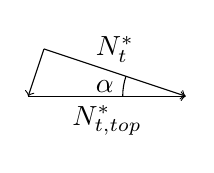
\begin{tikzpicture}[scale=.2]
\draw(6,0)arc(180:180-18.435:4)node[midway,left]{$\alpha$};
\draw[->](0,0)--++(10,0)node[midway,below]{$N^*_{t,top}$};
\draw[<-](10,0)--++(-9,3)node[midway,above]{$N^*_t$};
\draw[<-](0,0)--++(1,3);
\end{tikzpicture}
\end{figure}
\begin{flushright}
Use Grade 300 $\phi\SI{16}{\mm}$ rod
\end{flushright}
\end{solution}